
\noindent
\begin{tabular}{cc}
\begin{minipage}{0.60\textwidth}
%\sectionIf{\flagSect}{\taitol{Esercizio}}
\begin{exercise}[Leva idraulica]
La leva idraulica, rappresentata in figura, \`e formata da due
sistemi cilindro-pistone. 
Determinare la forza che \`e necessario applicare al secondo pistone 
per mantenere il sistema in equilibrio
quando sul primo agisce una forza $F_1 = 5000\ N$, 
allorch\'e i pistoni si trovano nella posizione indicata in figura.

Dati: diametro primo cilindro: $d_1 = 0.2\ m$; diametro secondo cilindro: 
$d_2 = 0.4\ m$; diametro del condotto che unisce i due cilindri:
$0.025\ m$;
densit\`a del fluido di lavoro: $600\ kg/m^3$;
altezza del primo pistone $h_1 = 1\ m$, altezza del secondo pistone
$h_2=2\ m$.\\ 
($p_1=159155\ Pa$, $p_2=153269\ Pa$, $\bm{F}_2=-19260.3 \hat{\bm{z}}\ N$.)
\end{exercise}
\end{minipage}
&
\begin{minipage}{0.35\textwidth}
   \begin{center}
   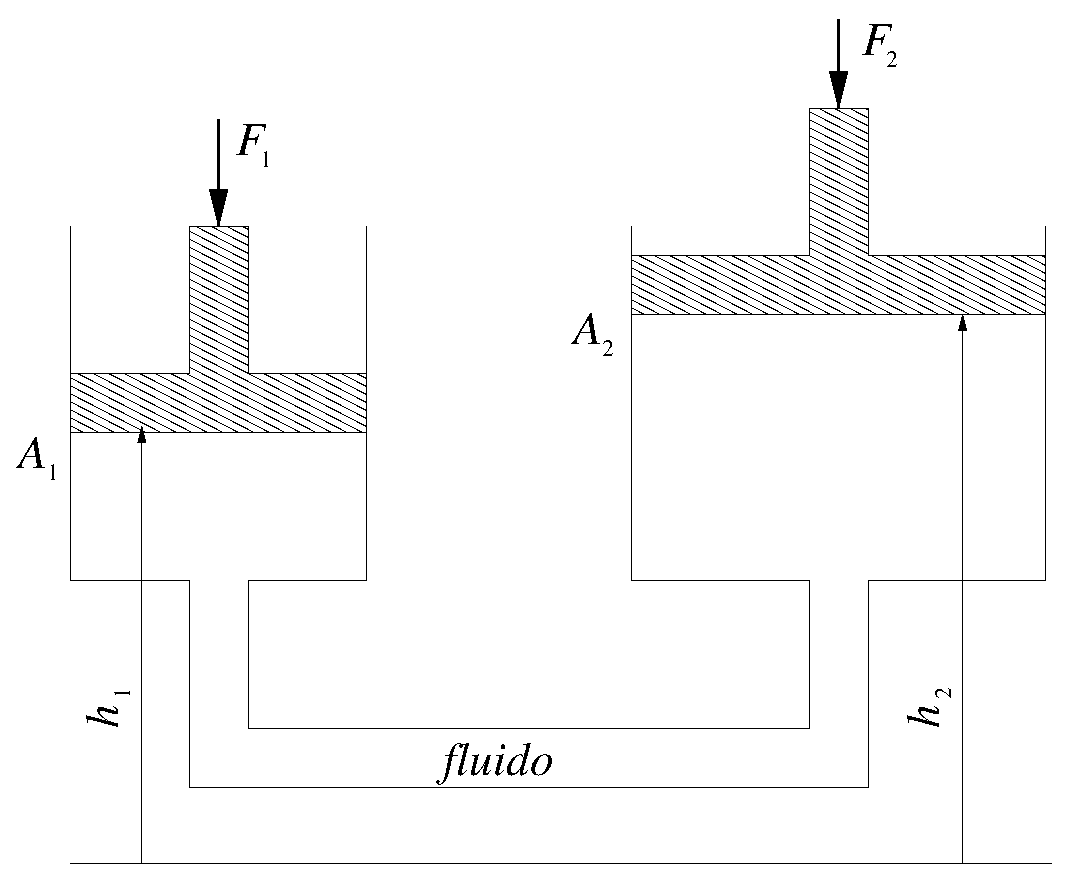
\includegraphics[width=0.90\textwidth]{./fig/leva_idraulica1.eps}
   \end{center}
\end{minipage}
\end{tabular}

\sol

\partone
 Legge di Stevino. Risultante statica. Leva idraulica.

\parttwo
 Il problema si risolve scrivendo le condizioni di equilibrio tra le forze esterne e la risultante dello sforzo di pressione sulle facce opposte dei pistoni e applicando la legge di Stevino tra le due sezioni $A_1$ e $A_2$.
Si ottiene un sistema lineare di tre equazioni in tre incognite $p_1, p_2, F_2$),
\begin{equation}
\begin{cases}
  F_1 = p_1 \pi \dfrac{d_1 ^2}{4} & \text{(Equilibrio pistone 1)} \\
  p_2 = p_1 - \rho g (h_2 - h_1) & \text{(Legge di Stevino)} \\
  F_2 = p_2 \pi \dfrac{d_2 ^2}{4} & \text{(Equilibrio pistone 2)} \ ,
\end{cases}
\end{equation}
la cui soluzione è
\begin{equation}
\Rightarrow \quad
\begin{cases}
  p_1 = \dfrac{4}{\pi} \dfrac{F_1}{d_1^2}  & = 159155 Pa \\
  p_2 = \dfrac{4}{\pi} \dfrac{F_1}{d_1^2} - \rho g (h_2 - h_1) & = 153269 Pa \\
  F_2 = \dfrac{d_1^2}{d_2^2} F_1 - \dfrac{\pi}{4}d_2^2 \ \rho g (h_2 - h_1) & = 19260.3  N \ .
\end{cases}
\end{equation}
La componente verticale $F_2$ della forza $\bm{F_2}$ è positiva diretta verso il basso, come nel disegno. Si  può scrivere quindi $\bm{F_2} = - F_2 \bm{\hat{z}}$, se il versore $\bm{\hat{z}}$ è orientato verso l'alto.
